\chapter{Diagramma delle classi}

\section{Definizione delle classi}

    \subsection*{1. Utente\_Non\_Loggato}
        La classe ``Utente\_Non\_Loggato'' rappresenta la classe di utenti che non hanno ancora effettuato l'accesso all'interno del sistema. Tale categoria di utenti ha accesso alle funzionalità di login e di visualizzazione dei dati forniti dalla zona visualizzata, i metodi presenti all'interno della classe stessa permettono di applicare le funzionalità precedentemente citate.
        \begin{figure}[H]
            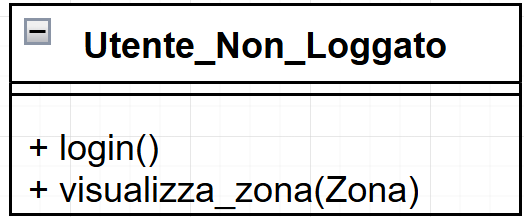
\includegraphics[width=0.3\textwidth]{ClassDiagram/Utente_Non_Loggato.png}
        \end{figure}     

    \subsection*{2. Utente}
        L'attore utente, da cui la classe omonima, rappresenta la classe astratta che viene estesa da tutte le tipologie di utenti presenti all'interno del programma. All'interno della classe ``Utente'' sono presenti i campi contenenti le informazioni personali ed i metodi comuni a tutti gli utenti, oppure necessari per definire il ruolo che l'utente ricopre all'interno del programma stesso.
        \begin{figure}[H]
            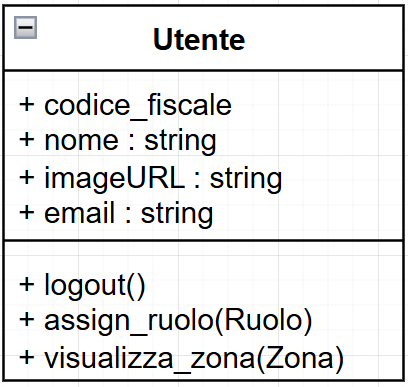
\includegraphics[width=0.3\textwidth]{ClassDiagram/Utente.png}
        \end{figure}

    \subsection*{3. Utente\_Analista}
        La classe ``Utente\_Analista'' raffigura la classe di utenti che hanno la possibilità di visualizzare una maggiore quantità di informazion e di statistiche al fine di analizzarne l'andamento e di studiare le strategie più efficaci per aumentare il grado di soddisfazione dei cittadini all'interno della città. La classe estende la classe ``Utente'', alla quale aggiunge gli attributi e i metodi necessari per gestire l'area di influenza dell'Analista stesso e i metodi per visualizzare in modo più dettagliato le informazioni contenute all'interno della classe ``Zona''.
        \begin{figure}[H]
            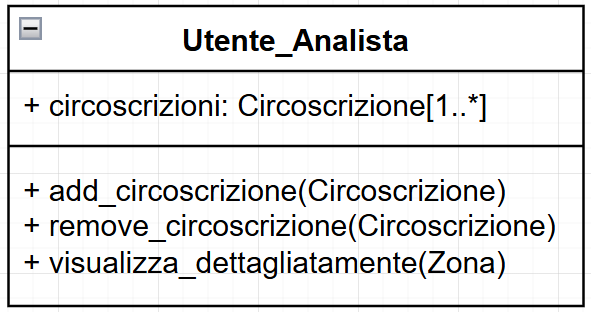
\includegraphics[width=0.3\textwidth]{ClassDiagram/Utente_Analista.png}
        \end{figure}

    \subsection*{4. Utente\_Sondaggista}
        La classe ``Utente\_Sondaggista'' raffigura la classe di utenti che hanno la possibilità di aggiungere o eliminare i sondaggi ed i voti presenti all'interno dei sondaggi stessi, permettendo ai cittadini la possibilità di esprimere il proprio grado di soddisfazione riguardo i servizi comunali e le politiche attutate dal comune. La classe estende la classe ``Utente'', alla quale aggiunge gli attributi e i metodi necessari per gestire i sondaggi, i voti e l'area di influenza del sondaggista stesso.
        \begin{figure}[H]
            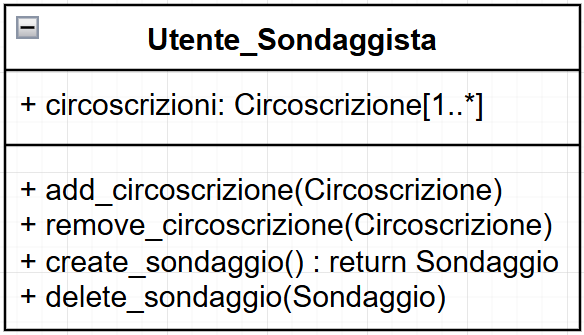
\includegraphics[width=0.3\textwidth]{ClassDiagram/Utente_Sondaggista.png}
        \end{figure}

    \subsection*{5. Utente\_Circoscrizione}
        La classe ``Utente\_Circoscrizione'' raffigura la classe di utenti che hanno la possibilità di gestire le funzionalità di maggiore rilievo all'interno della circoscrizione di appartenenza, tra le quali la gestione delle strutture, dei ruoli e delle richieste. La classe estende la classe ``Utente'', alla quale aggiunge gli attributi e i metodi necessari per le funzionalità di gestione delle strutture, dei ruoli e delle richieste.
        \begin{figure}[H]
            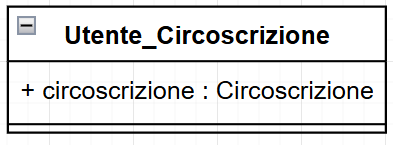
\includegraphics[width=0.3\textwidth]{ClassDiagram/Utente_Circoscrizione.png}
        \end{figure}

    \subsection*{6. Utente\_Amministratore}
        La classe ``Utente\_Amministratore'' raffigura la classe di utenti che hanno la possibilità di gestire le funzionalità di maggiore rilievo all'interno del comune di appartenenza, tra le quali la gestione delle strutture, dei ruoli, dell'approvazione dei sondaggi e delle risposte alle richieste da parte delle circoscrizioni. La classe estende la classe ``Utente'', alla quale aggiunge gli attributi e i metodi necessari per le funzionalità di gestione delle strutture, dei ruoli e delle risposte.
        \begin{figure}[H]
            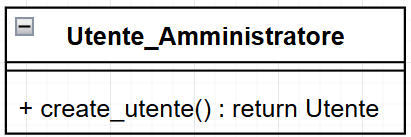
\includegraphics[width=0.3\textwidth]{ClassDiagram/Utente_Amministratore.png}
        \end{figure}

    \subsection*{7. Richiesta}
        La gestione delle richieste è identificata dalla classe omonima ``Richiesta'', tale classe permette di gestire il testo della richiesta, le informazioni riguardanti il mittente e la risposta fornita da uno degli utenti amministratore. Una volta completati i campi della richiesta e inviata la richiesta agli utenti amministratore la classe aspetterà una risposta da poter fornire all'utente circoscrizione da parte della classe ``Risposta''.
        \begin{figure}[H]
            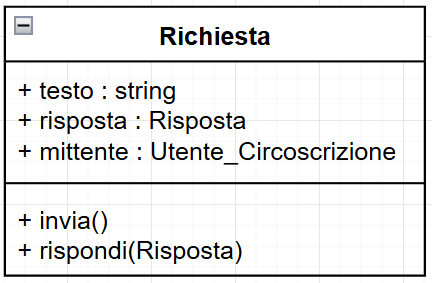
\includegraphics[width=0.3\textwidth]{ClassDiagram/Richiesta.png}
        \end{figure}
    
    \subsection*{8. Risposta}
        La gestione delle risposte è identificata dalla classe omonima ``Risposta'', tale classe permette di gestire la richiesta da parte dell'utente circoscrizione e il testo della relativa risposta. Una volta ricevuta la richiesta l'utente amministratore è in grado di fornire un relativo testo di risposta e successivamente inviare la risposta al mittente presente nella classe la classe ``Richiesta''.
        \begin{figure}[H]
            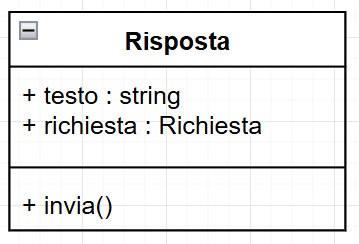
\includegraphics[width=0.3\textwidth]{ClassDiagram/Risposta.png}
        \end{figure}

    \subsection*{9. Sondaggio}
        Per la gestione dei sondaggi è stata identificata la classe omonima ``Sondaggio'', tale classe permette di gestire le informazioni che vengono caricare all'interno del sondaggio e le operazioni che vengono effettuate sul sondaggio stesso. L'utente sondaggista crea il sondaggio, successivamente sui sondaggi aperti sarà possibile aggiungere e rimuovere i voti, infine, successivamente alla chiusura del sondaggio, sarà possibile per gli utenti sondaggisti approvare o rifiutare i sondaggi stessi.
        \begin{figure}[H]
            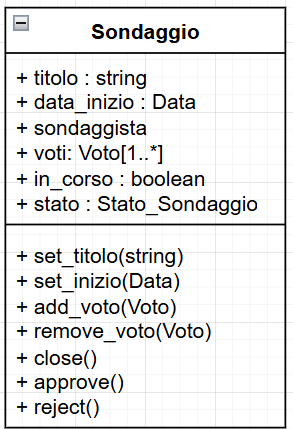
\includegraphics[width=0.3\textwidth]{ClassDiagram/Sondaggio.png}
        \end{figure}
    
    \subsection*{10. Voto}
        I voti presenti all'interno della classe ``Sondaggi'' sono appartenenti alla classe ``Voto'', tale classe ha lo scopo di memorizzare i dati generici, quali la circoscrizione di appartenenza e la fascia d'età, dei cittadini votanti oltre che il voto espresso attraverso un valore numerico.
        \begin{figure}[H]
            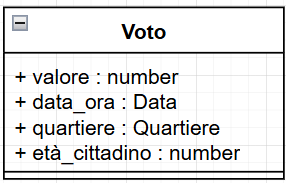
\includegraphics[width=0.3\textwidth]{ClassDiagram/Voto.png}
        \end{figure}

    \subsection*{11. Zona}
        La classe ``Zona'' rappresenta la classe astratta che viene estesa dalle diverse tipologie di zone geografiche che dividono la città, ovvero quartieri e circoscrizioni. All'interno della classe ``Zona'' sono presenti i campi contenenti le informazioni necessarie per distinguere e memorizzare le diverse zone geografiche oltre ai metodi necessari per gestire le strutture presenti all'interno dell'area geografica e per modificare alcuni dei campi presenti al suo interno.
        \begin{figure}[H]
            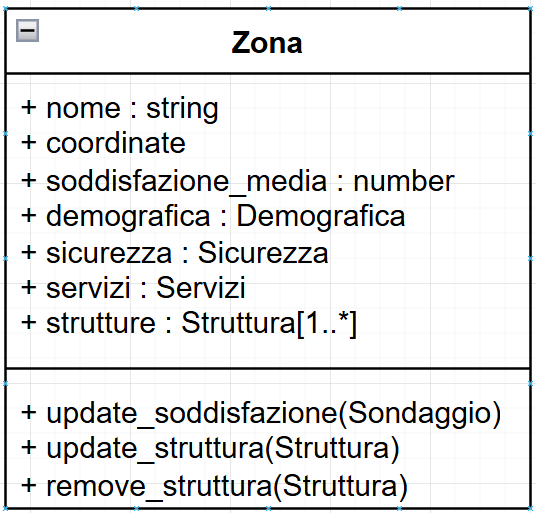
\includegraphics[width=0.3\textwidth]{ClassDiagram/Zona.png}
        \end{figure}

    \subsection*{12. Circoscrizione}
        La classe ``Circoscrizione'' estende la classe ``Zona'' in quanto questa definisce una zona di territorio specifica, la circoscrizione si compone, oltre che dai campi e dai metodi dalla classe padre, del campo ``Quartieri'' che tiene traccia delle classi ``Quartiere'' dalle quali questa è composta.
        \begin{figure}[H]
            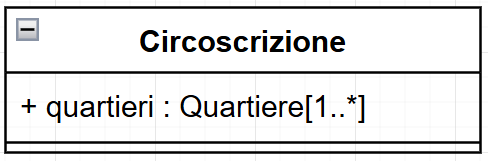
\includegraphics[width=0.3\textwidth]{ClassDiagram/Circoscrizione.png}
        \end{figure}
    
    \subsection*{13. Quartiere}
        La classe ``Quartiere'' estende la classe ``Zona'' in quanto questa definisce una zona di territorio specifica, il quartiere si compone, oltre che dai campi e dai metodi dalla classe padre, dai metodi necessari per modificare i campi presenti al suo interno.
        \begin{figure}[H]
            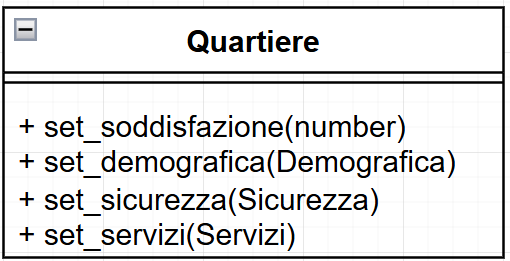
\includegraphics[width=0.3\textwidth]{ClassDiagram/Quartiere.png}
        \end{figure}
    
    \subsection*{14. Struttura}
        Per la gestione delle strutture è stata identificata la classe ``Struttura'' che servirà a gestire le informazioni riguardo alle strutture presenti all'interno delle diverse zone geografiche.
        \begin{figure}[H]
            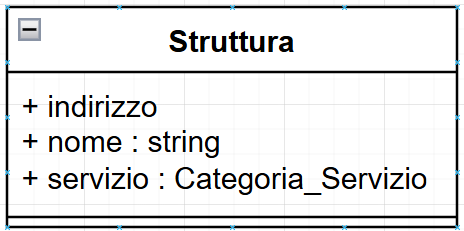
\includegraphics[width=0.3\textwidth]{ClassDiagram/Struttura.png}
        \end{figure}

\newpage
\section{Diagramma delle classi complessivo}
    Riportiamo di seguito il diagramma delle classi con tutte le classi fino ad ora presentate.
    \begin{figure}[H]
        \centering
        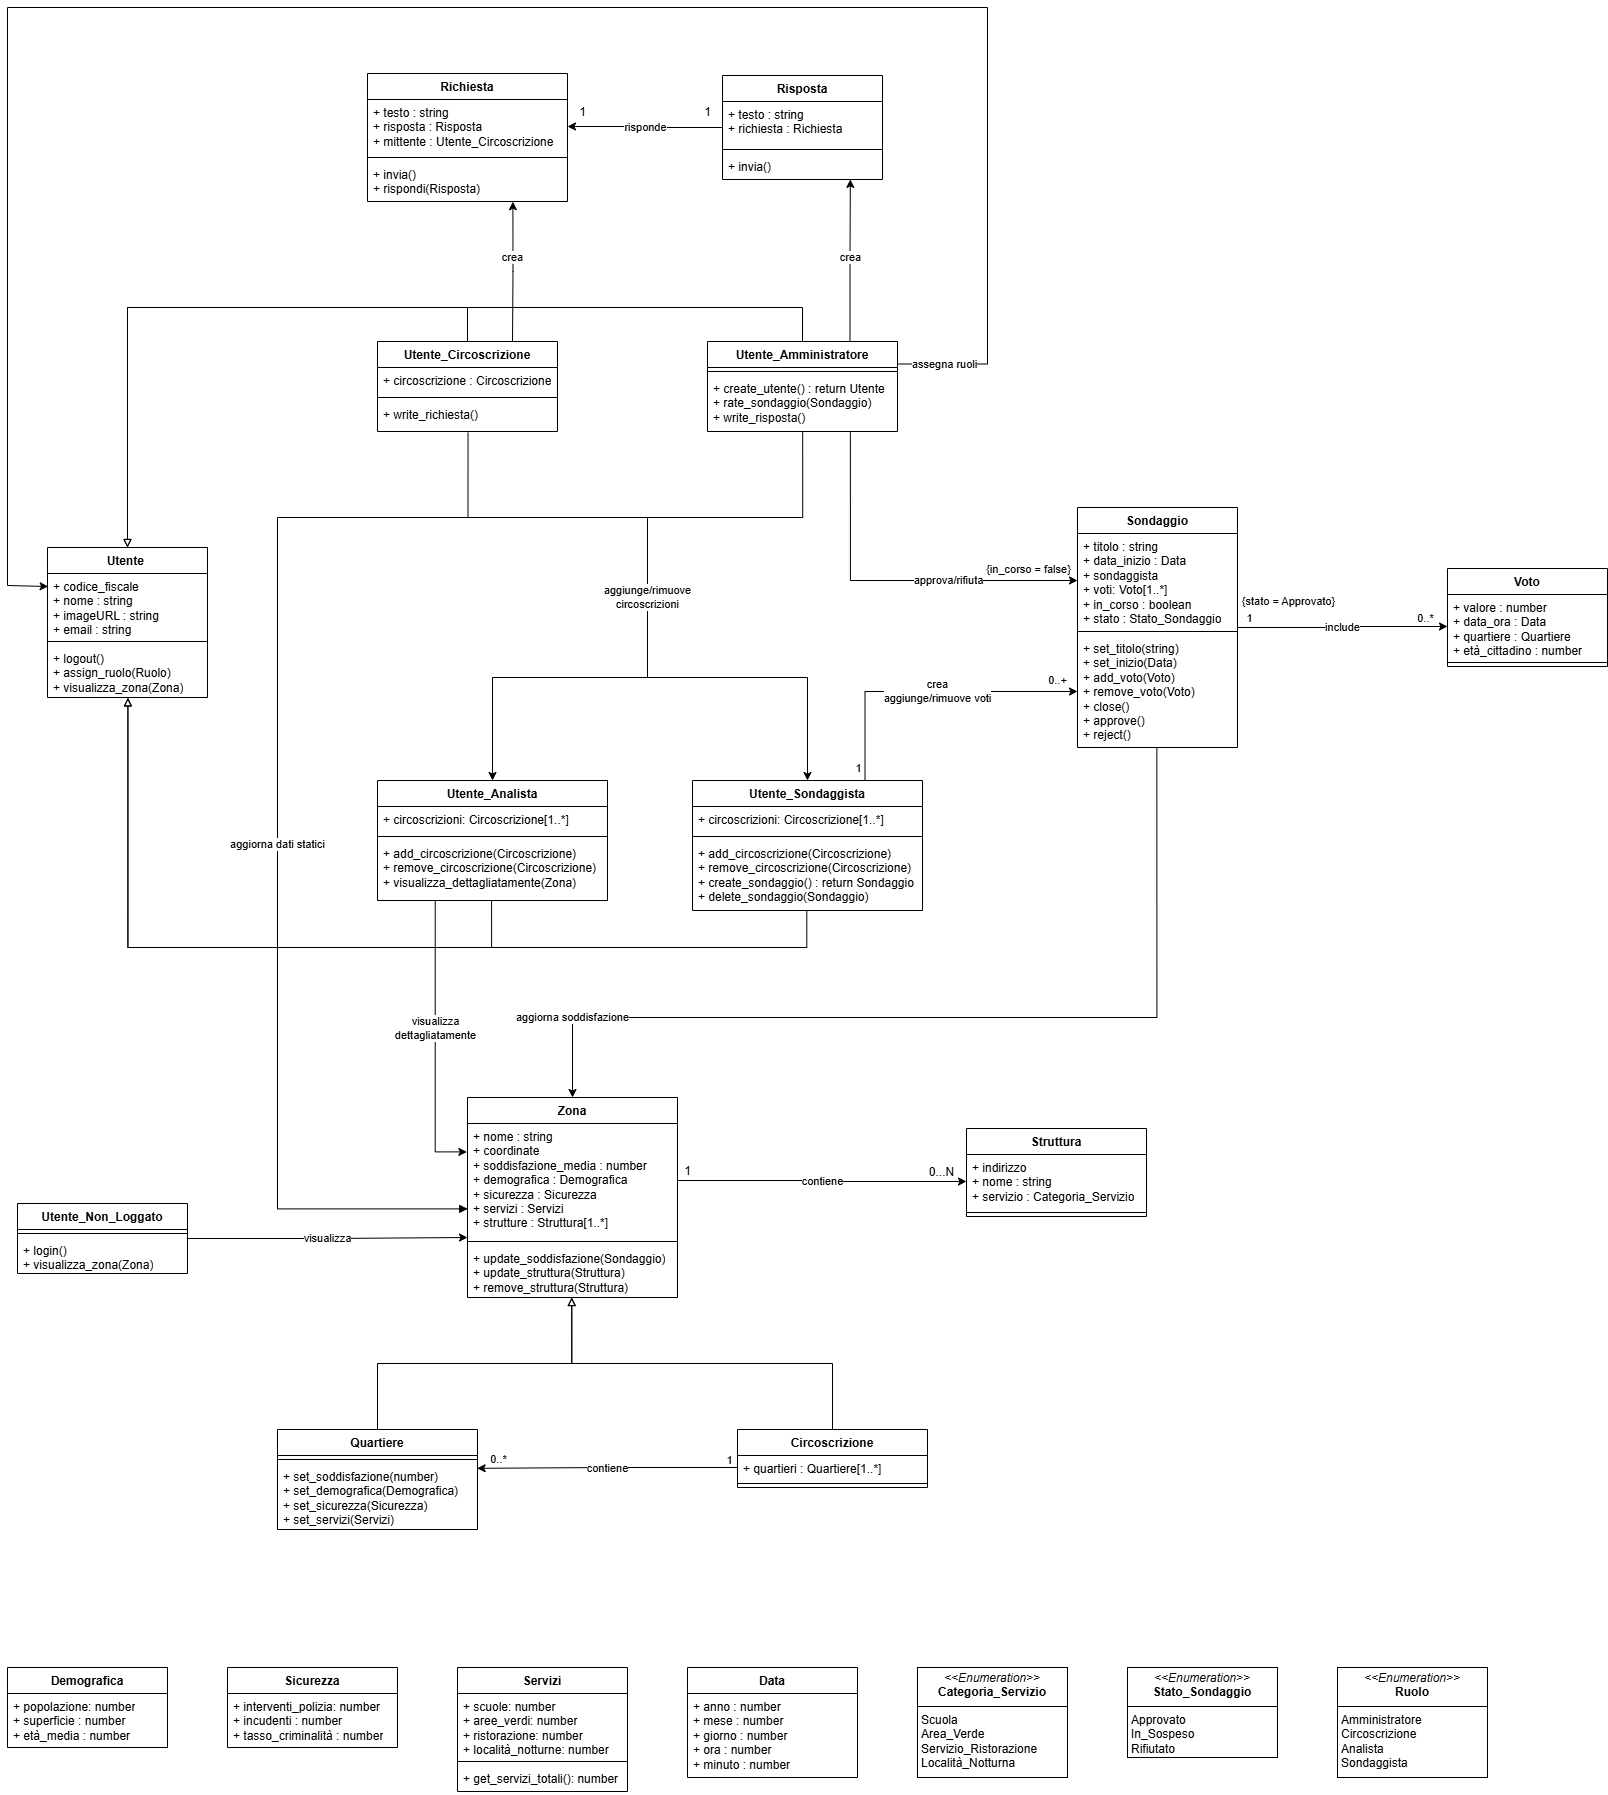
\includegraphics[width=1\textwidth]{ClassDiagram/ClassDiagram.drawio.png}
    \end{figure}